\chapter{La libreria \texttt{TireGround}}
\label{Codice}
%
\section{Organizzazione}
La libreria \texttt{TireGround} è stata organizzata in due parti, la prima gestisce la superficie stradale mentre la seconda gestisce i modelli di contatto dello pneumatico. Si sviluppa all'interno dell'omonimo \textit{namespace} \texttt{TireGround} nel quale vengono inoltre dichiarati con \texttt{typedef} alcuni tipi che verranno utilizzati nelle due sottosezioni. Verranno ora riportate le informazioni di maggior rilievo per ognuna delle due parti della libreria.

\subsection{Gestione della superficie stradale} 
La gestione della superficie stradale avviene all'interno del \textit{namespace} \texttt{RDF}. In quest'ultimo vengono raccolti alcuni tipi dichiarati con \texttt{typedef} presenti solo nel \textit{namespace} \texttt{RDF}. Lo spazio dei nomi \texttt{RDF} contiene tutti le classi e la funzioni per gestire e processare la \textit{mesh} a partire dal \textit{file} in formato \ac{RDF}.
%
\paragraph{\texttt{BBox2D}}
Questa classe contiene tutte le informazioni per definire, manipolare e processare una \ac{AABB} bidimensionale. Consiste nella descrizione geometrica dell'oggetto \ac{BB}. I metodi più importanti di questa classe sono i seguenti.
\begin{itemize}
	\item \texttt{clear} $-$ elimina il dominio della \ac{BB} settando tutti i quattro valori su \texttt{quietNaN}.
	\item \texttt{updateBBox2D} $-$ aggiorna il dominio della \ac{BB} settando i suoi valori secondo il massimo ingombro dato dai tre vertici nello spazio tridimensionale in \textit{input}.
\end{itemize}
\begin{table}[h!]
	\centering
	\begin{tabular}{|c|c|c|c|c|}
		\hline 
		\textbf{Tipo} & \textbf{Nome} & \textit{\textbf{Getter}} & \textit{\textbf{Setter}} & \textbf{Descrizione} \\ \hline 
		\texttt{real\_type} & \texttt{Xmin} & $\bullet$ & $\bullet$ & $X_{min}$ della \ac{AABB} \\ \hline 
		\texttt{real\_type} & \texttt{Ymin} & $\bullet$ & $\bullet$ & $Y_{min}$ della \ac{AABB} \\ \hline
		\texttt{real\_type} & \texttt{Xmax} & $\bullet$ & $\bullet$ & $X_{max}$ della \ac{AABB} \\ \hline
		\texttt{real\_type} & \texttt{Ymax} & $\bullet$ & $\bullet$ & $Y_{max}$ della \ac{AABB} \\ \hline
	\end{tabular}
	\caption{Attributi della classe \texttt{BBox2D}.}
	\label{BBox2D}
\end{table}
%
\paragraph{\texttt{Triangle3D}}
Questa classe contiene tutte le informazioni geometriche per definire, manipolare e processare un triangolo con vertici nello spazio tridimensionale. Consiste nella descrizione geometrica dell'oggetto triangolo. I metodi più importanti di questa classe sono:
\begin{itemize}
	\item \texttt{Normal} $-$ calcola la normale alla faccia del triangolo.
	\item \texttt{intersectRay} $-$ interseca il triangolo con una data semiretta (detta anche raggio), definita da direzione e punto di origine, e ne calcola il punto di intersezione.
	\item \texttt{intersectPlane} $-$ interseca il triangolo con un dato piano, definito da normale e punto noto e ne calcola i punti di intersezione.
\end{itemize}
\begin{table}[h!]
	\centering
	\begin{tabular}{|c|c|c|c|c|}
		\hline 
		\textbf{Tipo} & \textbf{Nome} & \textit{\textbf{Getter}} & \textit{\textbf{Setter}} & \textbf{Descrizione} \\ \hline 
		\texttt{vec3} & \texttt{Vertices[3]} & $\bullet$ & $\bullet$ & Vertici del triangolo \\ \hline 
		\texttt{vec3} & \texttt{Normal} & $\bullet$ & $\bullet$ & Normale al triangolo \\ \hline 
		\texttt{BBox2D} & \texttt{TriangleBBox} & $\bullet$ & $\bullet$ & \ac{AABB} del triangolo \\ \hline
	\end{tabular}
	\caption{Attributi della classe \texttt{Triangle3D}.}
\end{table}
%
\begin{figure}[h!]
	\centering
	\begin{tikzpicture}
	[
	grow                    = down,
	sibling distance    = 8em,
	level distance       = 4.5em,
	edge from parent/.style = {draw,stealth-},
	every node/.style       = {font=\footnotesize}
	]
	\node [root, env] {BBox2D}
	child { node [env] {Triangle3D}
		edge from parent node [right,tt] {TriangleBBox}  node [left,tt,color=white] {TriangleBBox} };
	\end{tikzpicture}	
	\caption{Diagramma delle collaborazioni per la classe \texttt{Triangle3D}.}
\end{figure}
\begin{figure}[h!]
	\centering
	\begin{tikzpicture}
	[
	grow                    = down,
	sibling distance    = 8em,
	level distance       = 4.5em,
	edge from parent/.style = {draw,stealth-},
	every node/.style       = {font=\footnotesize},
	sloped
	]
	\node [root, env] {Triangle3D}
	child { node [env] {TriangleRoad}
		edge from parent node [below,tt] {} };
	\end{tikzpicture}
	\caption{Diagramma dell'ereditarietà per la classe \texttt{Triangle3D}.}
\end{figure}
%
\paragraph{\texttt{TriangleRoad}}
Questa classe contiene tutte le informazioni geometriche e non geometriche per definire e manipolare un triangolo con vertici nello spazio tridimensionale rappresentante la superficie stradale. È derivato dalla classe \texttt{Triangle3D} e ha inoltre un attributo che permette di descrivere il coefficiente di attrito nella faccia. I metodi più importanti sono ereditati dalla classe \texttt{Triangle3D}.
%
\begin{table}[h!]
	\centering
	\begin{tabular}{|c|c|c|c|c|}
		\hline 
		\textbf{Tipo} & \textbf{Nome} & \textit{\textbf{Getter}} & \textit{\textbf{Setter}} & \textbf{Descrizione} \\ \hline 
		\texttt{real\_type} & \texttt{Friction} & $\bullet$ & $\bullet$ & Coefficiente di attrito $\mu$ \\ \hline
	\end{tabular}
	\caption{Attributi della classe \texttt{TriangleRoad}.}
\end{table}
%
\begin{figure}[h!]
	\centering
	\begin{tikzpicture}
	[
	grow                    = down,
	sibling distance    = 8em,
	level distance       = 4.5em,
	edge from parent/.style = {draw,stealth-},
	every node/.style       = {font=\footnotesize},
	]
	\node [root, env] {BBox2D}
	child { node [env] {Triangle3D}
		child { node [env] {TriangleRoad}
			edge from parent node [below,tt] {} }
		edge from parent node [right,tt] {TriangleBBox} node [left,tt,color=white] {TriangleBBox} };
	\end{tikzpicture}
	\caption{Diagramma delle collaborazioni per la classe \texttt{TriangleRoad}.}
\end{figure}[h!]
\begin{figure}\textbf{}
	\centering
	\begin{tikzpicture}
	[
	grow                    = down,
	sibling distance    = 8em,
	level distance       = 4.5em,
	edge from parent/.style = {draw,stealth-},
	every node/.style       = {font=\footnotesize},
	sloped
	]
	\node [root, env] {Triangle3D}
	child { node [env] {TriangleRoad}
		edge from parent node [below,tt] {} };
	\end{tikzpicture}
	\caption{Diagramma dell'ereditarietà per la classe \texttt{TriangleRoad}.}
\end{figure}
%
\paragraph{\texttt{MeshSurface}}
Questa classe contiene il vettore di puntatori di tipo \texttt{std::shared}-\texttt{\_ptr} alle istanze della classe \texttt{TriangleRoad} che vengono create durante l'analisi sintattico-grammaticale del \textit{file} \ac{RDF}. Inoltre, contiene il vettore di puntatori alle \ac{BB} di tipo \texttt{PtrBBox}, necessario per calcolare l'albero di tipo \ac{AABB}. Quest'ultimo esiste come ulteriore attributo della classe sotto forma di puntatore \texttt{PtrAABB}. I metodi più importanti di questa classe sono:
\begin{itemize}
	\item \texttt{set} $-$ copia la \textit{mesh} da un'altra già esistente.
	\item \texttt{LoadFile} $-$ effettua l'analisi sintattico-grammaticale del \textit{file} dato come \textit{input} e crea le istanze \texttt{TriangleRoad} che costituiscono la \textit{mesh}.
	\item \texttt{updateIntersection} $-$ interseca l'albero di tipo \ac{AABB} della \textit{mesh} con un altro albero esterno di tipo \ac{AABB} e ne restituisce il vettore dei puntatori di tipo \texttt{std::shared\_ptr} alle istanze della classe \texttt{TriangleRoad} che vengono intersecate.
\end{itemize}
\begin{table}[h!]
	\centering
	\begin{tabular}{|c|c|c|c|c|}
		\hline 
		\textbf{Tipo} & \textbf{Nome} & \textit{\textbf{Getter}} & \textit{\textbf{Setter}} & \textbf{Descrizione} \\ \hline 
		\texttt{TriangleRoad\_list} & \texttt{Friction} & $\bullet$ & & Vettore dei triangoli \\ \hline
		\texttt{std::vector<PtrBBox>} & \texttt{PtrBBoxVec} & $\bullet$ & & Vettore delle \ac{BB} \\ \hline
		\texttt{PtrAABB} & \texttt{PtrTree} & $\bullet$ & & Albero di tipo \ac{AABB} \\ \hline
	\end{tabular}
	\caption{Attributi della classe \texttt{MeshSurface}.}
\end{table}
%
\subsection{Gestione dei modelli di pneumatico} 
La gestione dei modelli di contatto dello pneumatico avviene nel \textit{namespace} \texttt{Tire}-\texttt{Ground}. Quest'ultimo contiene tutti le classi e la funzioni per gestire l'intersezione tra lo pneumatico e la \textit{mesh} a partire dalla conoscenza di quest'ultima, della geometria e della posizione dello pneumatico.
%
\paragraph{\texttt{Disk}}
Questa classe contiene tutte le informazioni geometriche per definire e manipolare un disco nello spazio tridimensionale. Consiste nella descrizione geometrica e nel posizionamento dello spazio delle coordinate tridimensionali dell'oggetto disco (il disco viene rappresentato nel sistema di riferimento dello pneumatico). I metodi più importanti di questa classe sono:
\begin{itemize}
	\item \texttt{isPointInside} $-$ controlla se un punto generico nello spazio bidimensionale, definito dal piano in cui giace lo stesso disco, si trova all'interno o all'esterno della circonferenza.
	\item \texttt{intersectSegment} $-$ trova i punti di intersezione tra la circonferenza esterna del disco e un segmento bidimensionale, che dev'essere definito nel piano in cui giace lo stesso disco. L'intero di \textit{output} fornisce il numero di punti di intersezione.
	\item \texttt{intersectPlane} $-$ interseca il disco con un piano definito da normale e punto noto. In \textit{output} fornisce l'entità geometrica creata dall'intersezione sotto forma di punto noto e direzione della retta.
	\item \texttt{contactTriangles} $-$ funzione in \textit{overloading} che consente di ottenere il versore normale e coefficiente attrito medi ponderati sull'area, nonché l'area di contatto stessa all'interno del singolo disco a partire da una serie di triangoli.
	\item \texttt{contactPlane} $-$ funzione in \textit{overloading} che consente di ottenere l'area di contatto all'interno del singolo disco dato un piano.
\end{itemize}
\begin{table}[h!]
	\centering
	\begin{tabular}{|c|c|c|c|c|}
		\hline 
		\textbf{Tipo} & \textbf{Nome} & \textit{\textbf{Getter}} & \textit{\textbf{Setter}} & \textbf{Descrizione} \\ \hline 
		\texttt{vec2} & \texttt{OriginXZ} & $\bullet$ & $\bullet$ & Coordinate \textit{XZ} del disco \\ \hline 
		\texttt{real\_type} & \texttt{OffsetY} & $\bullet$ & $\bullet$ & Coordinata $Y$ del disco \\ \hline
		\texttt{real\_type} & \texttt{Radius} & $\bullet$ & $\bullet$ & Raggio del disco \\ \hline
	\end{tabular}
	\caption{Attributi della classe \texttt{Disk}.}
	\label{}
\end{table}
%
\paragraph{\texttt{ETRTO}}
Questa classe contiene tutte le informazioni necessarie per definire geometricamente uno pneumatico secondo la normativa \ac{ETRTO}. Consiste nella descrizione geometrica dell'oggetto pneumatico in termini di larghezza totale e di diametro esterno indeformato. Come visto nel Capitolo \ref{Pneumatico} attraverso la nomenclatura \ac{ETRTO} (e.g. 205/65R16) è infatti possibile risalire a tutte le informazioni geometriche che definiscono, anche se in maniera grossolana, lo pneumatico.
\begin{table}[h!]
	\centering
	\begin{tabular}{|c|c|c|c|c|}
		\hline 
		\textbf{Tipo} & \textbf{Nome} & \textit{\textbf{Getter}} & \textit{\textbf{Setter}} & \textbf{Descrizione} \\ \hline 
		\texttt{real\_type} & \texttt{SectionWidth} & $\bullet$ & $\bullet$ & Larghezza dello pneumatico \\ \hline 
		\texttt{real\_type} & \texttt{AspectRatio} & $\bullet$ & $\bullet$ & Rapporto percentuale $H/W$ \\ \hline
		\texttt{real\_type} & \texttt{RimDiameter} & $\bullet$ & $\bullet$ & Diametro del cerchione\\ \hline
		\texttt{real\_type} & \texttt{SidewallHeight} & $\bullet$ & & Altezza della spalla \\ \hline
		\texttt{real\_type} & \texttt{TireDiameter} & $\bullet$ & & Diametro dello pneumatico\\ \hline
	\end{tabular}
	\caption{Attributi della classe \texttt{ETRTO}.}
	\label{}
\end{table}
%
\paragraph{\texttt{ReferenceFrame}}
Questa classe contiene tutte le informazioni per definire e manipolare una terna di riferimento nello spazio tridimensionale. Consiste nel posizionamento dello spazio del sistema di riferimento. I metodi più importanti di questa classe sono:
\begin{itemize}
	\item \texttt{setTotalTransformationMatrix} $-$ posiziona nello spazio il sistema di riferimento grazie alla matrice di trasformazione $4\times4$ fornita come \textit{input}.
	\item \texttt{getEulerAngleX} $-$ ottiene l'angolo creato dalla rotazione attorno all'asse $Y$ del sistema di riferimento locale rispetto a quello assoluto (lo stesso della \textit{mesh}). L'angolo viene ottenuto in seguito alla fattorizzazione $R_z(\Omega) R_x(\gamma) R_y(\theta)$ e utilizzando il metodo di Eulero.
	\item \texttt{getEulerAngleY} $-$ come il metodo \texttt{getEulerAngleX}, ma usato per ottenere l'angolo creato dalla rotazione attorno all'asse $Y$.
	\item \texttt{getEulerAngleZ} $-$ come il metodo \texttt{getEulerAngleX}, ma usato per il ottenere l'angolo creato dalla rotazione attorno all'asse $Z$.
\end{itemize}
\begin{table}[h!]
	\centering
	\begin{tabular}{|c|c|c|c|c|}
		\hline 
		\textbf{Tipo} & \textbf{Nome} & \textit{\textbf{Getter}} & \textit{\textbf{Setter}} & \textbf{Descrizione} \\ \hline 
		\texttt{vec3} & \texttt{Origin} & $\bullet$ & $\bullet$ & Origine della terna \\ \hline 
		\texttt{mat3} & \texttt{RotationMatrix} & $\bullet$ & $\bullet$ & Matrice di rotazione \\ \hline
	\end{tabular}
	\caption{Attributi della classe \texttt{ReferenceFrame}.}
	\label{}
\end{table}
%
\paragraph{\texttt{Shadow}}
Questa classe serve a rappresentare l'ombra dello pneumatico nello spazio bidimensionale. È molto simile alla \texttt{RDF::BBox2D} precedentemente presentata, ma a differenza di quest'ultima permette di calcolare gli alberi di tipo \ac{AABB} relativi all'ombra totale, della parte superiore e della parte inferiore del \ac{BB} tridimensionale che racchiude lo pneumatico. I metodi più importanti di questa classe sono:
\begin{itemize}
	\item \texttt{clear} $-$ elimina il dominio dell'ombra settando tutti i suoi valori su \texttt{quietNaN}.
	\item \texttt{update} $-$ aggiorna il dominio dell'ombra settando tutti i suoi valori secondo il massimo ingombro dato dalla geometria dello pneumatico e dalla sua posizione nello spazio.
\end{itemize}
\begin{table}[h!]
	\centering
	\begin{tabular}{|c|c|c|c|c|}
		\hline 
		\textbf{Tipo} & \textbf{Nome} & \textit{\textbf{Getter}} & \textit{\textbf{Setter}} & \textbf{Descrizione} \\ \hline 
		\texttt{PtrAABB} & \texttt{PtrTree} & $\bullet$ & & Albero \ac{AABB} totale\\ \hline
		\texttt{PtrAABB} & \texttt{PtrTree\_U} & $\bullet$ & & Albero \ac{AABB} parte superiore \\ \hline
		\texttt{PtrAABB} & \texttt{PtrTree\_L} & $\bullet$ & & Albero \ac{AABB} parte inferiore \\ \hline
	\end{tabular}
	\caption{Attributi della classe \texttt{Shadow}.}
	\label{}
\end{table}
%
\paragraph{\texttt{SamplingGrid}}
Questa classe contiene tutti i parametri che riguardano la precisione dei calcoli che verranno effettuati nel calcolo della normale al terreno, punto e area di contatto.

Un attributo molto importante è \texttt{Switch}, esso consiste nel limite massimo di triangoli di tipo \texttt{TriangleRoad} che possono essere contenuti all'interno dell'ombra dello pneumatico prima di passare:
\begin{itemize}
	\item dal modello di contatto ponderato in base all'area d'intersezione al modello di contatto di Rill nel caso di pneumatico di tipo \texttt{MagicFormula};
	\item dal modello di contatto ponderato in base all'area d'intersezione al modello di contatto tramite campionamento nel caso di pneumatico di tipo \texttt{MultiDisk}.
\end{itemize}
Modificando il suo valore si può quindi decidere che tipo di modello di contatto adottare in base al numero di triangoli totali all'interno dell'ombra dello pneumatico. In questo modo, se la \textit{mesh} è estremamente fitta (100/200+ triangoli), si eviterà rallentare troppo l'esecuzione. Come si vedrà successivamente infatti, sia per quanto riguarda la precione dell'\textit{output} che per i tempi di esecuzione, converrà sempre utilizzare un modello di contatto di tipo ponderato in base all'area d'intersezione.
%
\begin{table}[h!]
	\centering
	\begin{tabular}{|c|c|c|c|c|}
		\hline 
		\textbf{Tipo} & \textbf{Nome} & \textit{\textbf{Getter}} & \textit{\textbf{Setter}} & \textbf{Descrizione} \\ \hline 
		\texttt{int\_type} & \texttt{PointsN} & $\bullet$ & $\bullet$ & N° di punti di campionamento \\ \hline 
		\texttt{int\_type} & \texttt{DisksN} & $\bullet$ & $\bullet$ & N° di dischi \\ \hline 
		\texttt{int\_type} & \texttt{Switch} & $\bullet$ & $\bullet$ & \textit{Threshold} per il tipo contatto \\ \hline
	\end{tabular}
	\caption{Attributi della classe \texttt{SamplingGrid}.}
	\label{}
\end{table}
%
\paragraph{\texttt{Tire}}
Questa classe serve a rappresentare lo pneumatico nelle coordinate dello spazio tridimensionale. Consiste nel punto di giunzione tra la classe \texttt{ETRTO} che definisce la geometria dello pneumatico in condizione di riposo e la classe \texttt{Reference}-\texttt{Frame} che ne definisce invece la posizione nello spazio. È una classe virtuale in quanto viene definita con alcuni metodi puri virtuali. Questi metodi verranno poi sostituiti con nelle classi figlie.
%
\begin{table}[h!]
	\centering
	\begin{tabular}{|c|c|c|c|c|}
		\hline 
		\textbf{Tipo} & \textbf{Nome} & \textit{\textbf{Getter}} & \textit{\textbf{Setter}} & \textbf{Descrizione} \\ \hline 
		\texttt{SamplingGrid} & \texttt{Precision} & & & Precisione dei calcoli \\ \hline 
		\texttt{ETRTO} & \texttt{TireGeometry} & & & Geometria \\ \hline 
		\texttt{ReferenceFrame} & \texttt{RF} & $\bullet$ & $\bullet$ & Posizione \\ \hline
	\end{tabular}
	\caption{Attributi della classe \texttt{Tire}.}
	\label{}
\end{table}
%
\begin{figure}[h!]
	\centering
	\begin{tikzpicture}
	[
	grow                    = down,
	sibling distance    = 8em,
	level distance       = 8.5em,
	edge from parent/.style = {draw,-stealth},
	every node/.style       = {font=\footnotesize},
	sloped
	]
	\node [root, env] {Tire}
	child { node [env] {SamplingGrid}
		edge from parent node [below,tt] {Precision} }
	child { node [env] {ETRTO}
		edge from parent node [below,tt] {TireGeometry} }
	child { node [env] {Shadow}
		edge from parent node [below,tt] {TireShadow} }
	child { node [env] {ReferenceFrame}
		edge from parent node [below,tt] {RF} };
	\end{tikzpicture}
	\caption{Diagramma delle collaborazioni per la classe \texttt{Tire}.}
\end{figure}
\begin{figure}[h!]
	\centering
	\begin{tikzpicture}
	[
	grow                    = down,
	sibling distance    = 8em,
	level distance       = 4.5em,
	edge from parent/.style = {draw,stealth-},
	every node/.style       = {font=\footnotesize},
	sloped
	]
	\node [root, env] {Tire}
	child { node [env] {MultiDisk}
		edge from parent node [below,tt] {} }
	child { node [env] {MagicFormula}
		edge from parent node [below,tt] {} };
	\end{tikzpicture}
	\caption{Diagramma dell'ereditarietà per la classe \texttt{Tire}.}
\end{figure}
%
\paragraph{\texttt{MagicFormula} e \texttt{MultiDisk}}
Queste classi calcolano tutti i parametri necessari per valutare il contatto tra pneumatico a disco singolo e terreno attraverso la formula di Pacejka. I metodi più importanti di queste classi sono:
\begin{itemize}
	\item \texttt{setup} $-$ consente di riposizionare la ruota all'interno della \textit{mesh};
	\item \texttt{getRelativeCamber} $-$ calcola il camber relativo;
	\item \texttt{getRho} $-$ calcola l'affondamento del disco nel piano strada locale;
	\item \texttt{getFriction} $-$ calcola il coefficiente di attrito nel punto di contatto;
	\item \texttt{getArea} $-$ calcola l'area d'intersezione dei dischi.
\end{itemize}
%
\begin{table}[h!]
	\centering
	\begin{tabular}{|c|c|c|c|}
		\hline 
		\textbf{Tipo} & \textbf{Nome} & \textit{\textbf{Getter}} & \textbf{Descrizione} \\ \hline 
		\texttt{Disk} & \texttt{SingleDisk} &  & Disco rigido \\ \hline 
		\texttt{vec3} & \texttt{Normal} & $\bullet$ & Versore del piano strada \\ \hline
		\texttt{vec3} & \texttt{MeshPoint} & $\bullet$ & Punto di contatto sulla \textit{mesh} \\ \hline
		\texttt{vec3} & \texttt{MeshPoint} & $\bullet$ & Punto di contatto sul disco \\ \hline
		\texttt{real\_type} & \texttt{Friction} & $\bullet$ & Coefficiente di attrito locale \\ \hline
		\texttt{real\_type} & \texttt{Area} & $\bullet$ & Area d'intersezione \\ \hline
	\end{tabular}
	\caption{Attributi della classe \texttt{MagicFormula}.}
	\label{}
\end{table}
%
\begin{table}[h!]
	\centering
	\begin{tabular}{|c|c|c|c|}
		\hline 
		\textbf{Tipo} & \textbf{Nome} & \textit{\textbf{Getter}} & \textbf{Descrizione} \\ \hline 
		\texttt{Disk} & \texttt{DiskVec} &  & Vettore dei dischi \\ \hline 
		\texttt{vec3} & \texttt{NormalVec} & $\bullet$ & Vettore dei versori normali \\ \hline
		\texttt{vec3} & \texttt{MeshPointVec} & $\bullet$ & Vettore dei punti di contatto sulla \textit{mesh} \\ \hline
		\texttt{vec3} & \texttt{DiskPointVec} & $\bullet$ & Vettore dei punti di contatto sul disco \\ \hline
		\texttt{real\_type} & \texttt{FrictionVec} & $\bullet$ & Vettore dei coefficienti di attrito locale \\ \hline
		\texttt{real\_type} & \texttt{AreaVec} & $\bullet$ & Vettore delle aree d'intersezione \\ \hline
		\texttt{vec3} & \texttt{Normal} & $\bullet$ & Versore del piano strada \\ \hline
		\texttt{vec3} & \texttt{MeshPoint} & $\bullet$ & Punto di contatto singolo sulla \textit{mesh} \\ \hline
		\texttt{vec3} & \texttt{MeshPoint} & $\bullet$ & Punto di contatto singolo sul disco \\ \hline
		\texttt{real\_type} & \texttt{Friction} & $\bullet$ & Coefficiente di attrito locale \\ \hline
		\texttt{real\_type} & \texttt{Area} & $\bullet$ & Area totale d'intersezione \\ \hline
	\end{tabular}
	\caption{Attributi della classe \texttt{MultiDisk}.}
	\label{}
\end{table}
%
\begin{figure}[h!]
	\centering
	\begin{tikzpicture}
		[
		grow                    = down,
		sibling distance    = 8em,
		level distance       = 8.5em,
		edge from parent/.style = {draw,-stealth},
		every node/.style       = {font=\footnotesize},
		sloped
		]
		\node [root, env] {MagicFormula}
		child { node [env] {Tire}
			child { node [env] {SamplingGrid}
				edge from parent node [below,tt] {Precision} }
			child { node [env] {ETRTO}
				edge from parent node [below,tt] {TireGeometry} }
			child { node [env] {Shadow}
				edge from parent node [below,tt] {TireShadow} }
			child { node [env] {ReferenceFrame}
				edge from parent node [below,tt] {RF} }
			edge from parent node [below,tt] {} }
		child { node [env] {Disk}
			edge from parent node [below,tt] {SingleDisk} };
	\end{tikzpicture}
	\caption{Diagramma delle collaborazioni per la classe \texttt{MagicFormula}.}
\end{figure}
\begin{figure}[h!]
	\centering
	\begin{tikzpicture}
	[
	grow                    = up,
	sibling distance    = 8em,
	level distance       = 4.5em,
	edge from parent/.style = {draw,-stealth},
	every node/.style       = {font=\footnotesize},
	sloped
	]
	\node [root, env] {MagicFormula}
	child { node [env] {Tire}
		edge from parent node [below,tt] {} };
	\end{tikzpicture}
	\caption{Diagramma dell'ereditarietà per la classe \texttt{MagicFormula}.}
\end{figure}
%
\begin{figure}[h!]
	\centering
	\begin{tikzpicture}
	[
	grow                    = down,
	sibling distance    = 8em,
	level distance       = 8.5em,
	edge from parent/.style = {draw,-stealth},
	every node/.style       = {font=\footnotesize},
	sloped
	]
	\node [root, env] {MultiDisk}
	child { node [env] {Tire}
		child { node [env] {SamplingGrid}
			edge from parent node [below,tt] {Precision} }
		child { node [env] {ETRTO}
			edge from parent node [below,tt] {TireGeometry} }
		child { node [env] {Shadow}
			edge from parent node [below,tt] {TireShadow} }
		child { node [env] {ReferenceFrame}
			edge from parent node [below,tt] {RF} }
		edge from parent node [below,tt] {} }
	child { node [env] {Disk}
		edge from parent node [below,tt] {DiskVec} };
	\end{tikzpicture}
	\caption{Diagramma delle collaborazioni per la classe \texttt{MultiDisk}.}
\end{figure}
\begin{figure}[h!]
	\centering
	\begin{tikzpicture}
	[
	grow                    = up,
	sibling distance    = 8em,
	level distance       = 4.5em,
	edge from parent/.style = {draw,-stealth},
	every node/.style       = {font=\footnotesize},
	sloped
	]
	\node [root, env] {MultiDisk}
	child { node [env] {Tire}
		edge from parent node [below,tt] {} };
	\end{tikzpicture}
	\caption{Diagramma dell'ereditarietà per la classe \texttt{MultiDisk}.}
\end{figure}
%
\clearpage
%
\section{Librerie ausiliarie}
Oltre al codice appena descritto sono state utilizzate anche altre due librerie esterne al fine di velocizzare il processo di sviluppo e al contempo di utilizzare una solida base per le operazione più complesse, ovvero le operazioni matriciali e vettoriali, nonché la creazione degli alberi per oggetti di tipo \ac{AABB} e l'intersezione tra gli stessi.
%
\subsection{\texttt{Eigen3}}
\texttt{Eigen3} è una libreria \texttt{C++} di alto livello di \textit{template headers} per operazioni di algebra lineare, vettoriali, matriciali, trasformazioni geometriche, \textit{solver} numerici e algoritmi correlati.

Questa libreria è ulizza la tecnica di \textit{template metaprogramming}, che crea degli alberi di espressioni in fase di compilazione e genera un codice ottimizzato per valutarli.
%
\subsection{\texttt{Clothoids}}
Questa libreria nasce per il \textit{fitting} e manipolazione di clotoidi, \textit{spline} di clotoidi, archi circolari e \textit{biarc}. In questo lavoro di tesi la libreria \texttt{Clothoids} è stata usata per sfruttare l'implementazione degli oggetti di tipo \ac{AABB} e del relativo albero.
%
\section{Esempi di uso della libreria}
La libreria \texttt{TireGround} è stata pensata per essere semplice da utilizzare. Si vedranno ora i vari passi per utilizzarla in maniera appropriata.
%
\paragraph{Caricare la \textit{mesh}}
Per caricare la superficie stradale, rappresentata dalla \textit{mesh} triangolare contenuta nel \textit{file} \ac{RDF}, è sufficiente sfruttare il costruttore della classe \texttt{Mesh}-\texttt{Surface} che prende in \textit{input} l'indirizzo al \textit{file}.
\begin{pseudoc}
	RDF::MeshSurface Road("./file.rdf");
\end{pseudoc}
%
\paragraph{Creare lo pneumatico}
Per creare lo pneumatico a singolo disco è sufficiente utilizzare il costruttore di \textit{default} della classe \texttt{MagicFormula}.
\begin{pseudoc}
	TireGround::Tire* SampleTire = new TireGround::MagicFormula(
		SectionWidth, // Sezione laterale dello pneumatico [m]
		AspectRatio,  // Aspect ratio percentuale dello pneumatico
		RimDiameter,  // Diametro del cerchio [in]
		SwitchNumber  // Threshold per passare dal modello di contatto ponderato in base all'area di intersezione a quello di Rill 
		);
\end{pseudoc}
Nel caso invece si voglia creare uno pneumatico a più dischi si utilizzerà uno dei costruttori della classe \texttt{MultiDisk}.

Per il caso di pneumatico a più dischi con raggio uniforme si avrà:
\begin{pseudoc}
	TireGround::Tire* SampleTire = new TireGround::MultiDisk(
		SectionWidth, // Sezione laterale dello pneumatico [m]
		AspectRatio,  // Aspect ratio percentuale dello pneumatico
		RimDiameter,  // Diametro del cerchio [in]
		PointsNumber, // Numero di punti di campionamento per ogni disco
		DisksNumber,  // Numero di dischi totale
		SwitchNumber  // Threshold per passare dal modello di contatto ponderato in base all'area di intersezione a quello di Rill 
		);
\end{pseudoc}
Nel caso di pneumatico a più dischi con raggio di raccordo sulla spalla si avrà invece:
\begin{pseudoc}
	TireGround::Tire* SampleTire = new TireGround::MultiDisk(
		SectionWidth, // Sezione laterale dello pneumatico [m]
		AspectRatio,  // Aspect ratio percentuale dello pneumatico
		RimDiameter,  // Diametro del cerchio [in]
		SideRadius,   // Raggio di raccordo sulla spalla [m]
		PointsNumber, // Numero di punti di campionamento per ogni disco
		DisksNumber,  // Numero di dischi totale
		SwitchNumber  // Threshold per passare dal modello di contatto ponderato in base all'area di intersezione a quello di Rill 
		);
\end{pseudoc}
Infine, nel caso si voglia creare uno pneumatico a più dischi con forma personalizzata:
\begin{pseudoc}
	TireGround::Tire* SampleTire = new TireGround::MultiDisk(
		SectionWidth, // Sezione laterale dello pneumatico [m]
		AspectRatio,  // Aspect ratio percentuale dello pneumatico
		RimDiameter,  // Diametro del cerchio [in]
		RadiusVec,    // Vettore dei raggi dei dischi [m]
		PointsNumber, // Numero di punti di campionamento per ogni disco
		SwitchNumber  // Threshold per passare dal modello di contatto ponderato in base all'area di intersezione a quello di Rill 
		);
\end{pseudoc}
%
\paragraph{Orientazione dello pneumatico e valutazione del contatto}
Per orientare lo pneumatico e valutarne il contatto con il manto stradale si utilizzerà il metodo \texttt{setup} della classe \texttt{Tire}.
\begin{pseudoc}
bool Out = TireMD->setup(
	Road, // Superficie stradale
	TM    // Matrice di trasformazione 4x4 per orientare lo pneumatico
	);
\end{pseudoc}
Per estrarre i risultati si andranno dapprima a inizializzazione delle variabili reali o vettoriali come segue.
\begin{pseudoc}
	// Inizializzazione delle variabili
	TireGround::vec3 N;
	TireGround::vec3 P;
	TireGround::real_type Friction;
	TireGround::real_type Rho;
	TireGround::real_type RhoDot;
	TireGround::real_type RelativeCamber;
	TireGround::real_type Area;
	TireGround::real_type Volume;
	
	// Estrazione della dimensione appropriata della struttura dati
	TireGround::int_type size = TireSD->getDisksNumber();
	
	// Inizializzazione dei vettori con dimensione appropriata
	TireGround::row_vec3 NVec(size);
	TireGround::row_vec3 PVec(size);
	TireGround::row_vecN FrictionVec(size);
	TireGround::row_vecN RhoVec(size);
	TireGround::row_vecN RhoDotVec(size);
	TireGround::row_vecN RelativeCamberVec(size);
	TireGround::row_vecN AreaVec(size);
	TireGround::row_vecN VolumeVec(size);
\end{pseudoc}
Successivamente verranno modificate dai metodi della classe \texttt{Tire} come:
\begin{pseudoc}
	// Estrazione dei dati
	SampleTire->getNormal(N);
	SampleTire->getMFpoint(P);
	SampleTire->getFriction(Friction);
	SampleTire->getRho(Rho);
	SampleTire->getRhoDot(PreviousRho,TimeStep,RhoDot);
	SampleTire->getRelativeCamber(RelativeCamber);
	SampleTire->getArea(Area);
	SampleTire->getVolume(Volume);
	
	// Estrazione dei dati in vettori
	SampleTire->getNormal(NVec);
	SampleTire->getMFpoint(PVec);
	SampleTire->getFriction(FrictionVec);
	SampleTire->getRho(RhoVec);
	SampleTire->getRhoDot(PreviousRho,TimeStep,RhoDotVec);
	SampleTire->getRelativeCamber(RelativeCamberVec);
	SampleTire->getArea(AreaVec);
	SampleTire->getVolume(VolumeVec);
\end{pseudoc}
%
\paragraph{Casi particolari}
Nel caso in cui la variabile booleana in \textit{output} dal metodo \texttt{setup} precedentemente chiamato sia falsa, si prospettano due casi.
%
\paragraph{Pneumatico fuori \textit{mesh}}
Per verificare questa consizione occorre intersecare l'albero della \textit{mesh} con l'albero a una foglia dell'ombra dello pneumatico.
\begin{pseudoc}
	RDF::TriangleRoad_list TrianglesList;
	bool List = Road.intersectAABBtree(TireSD->getAABBtree(), TrianglesList);
\end{pseudoc}
Se la variabile booleana in \textit{output} dal metodo \texttt{intersectAABBtree} è falsa allora la lista è vuota e lo pneumatico sarà quindi considerato fuori dalla superficie stradale descritta nel \textit{file} \ac{RDF}.
%
\paragraph{Pneumatico in volo}
Per verificare questa consizione occorre ancora intersecare l'albero della \textit{mesh} con l'albero a una foglia dell'ombra dello pneumatico.
\begin{pseudoc}
	RDF::TriangleRoad_list TrianglesList;
	bool List = Road.intersectAABBtree(TireSD->getAABBtree(), TrianglesList);
\end{pseudoc}
Se la variabile booleana in \textit{output} dal metodo \texttt{intersectAABBtree} è vera allora la lista non è vuota e lo pneumatico sarà quindi considerato in volo sopra la superficie stradale descritta nel \textit{file} \ac{RDF}. In questo caso i parametri d'intersezione vanno settati come intersezione nulla.
%
%
\section{Prestazioni della libreria}
I vari modelli di contatto sono stati preventivamente testati in una macchina avente le seguenti specifiche tecniche:
\begin{itemize}
	\item memoria RAM:
	\begin{itemize}
		\item dimensione: 8 GB;
		\item frequenza: 1.33 GHz;
	\end{itemize}
	\item processore:
	\begin{itemize}
		\item denominazione: Intel i5 3230M;
		\item numero di \textit{core}: 2;
		\item numero di thread: 4;
		\item frequenza base: 2.60 GHz;
		\item frequenza massima: 3.20 GHz;
		\item \textit{cache}: L3 3 MB.
	\end{itemize}
\end{itemize}
I tempi rilevati per il modello di pneumatico a singolo disco \texttt{MagicFormula} sono riportati nelle Tabelle \ref{MFcordolo} e \ref{MFpiano}. Analogamente, i tempi rilevati per il modello di pneumatico a più dischi \texttt{MultiDisk} sono riportati nelle Tabelle \ref{MDcordolo} e \ref{MDpiano}. Notare che le Tabelle \ref{MFcordolo} e \ref{MDcordolo} sono relative ad un'area dove la \textit{mesh} è più densa, mentre le Tabelle \ref{MFpiano} e \ref{MDpiano} sono relative ad un'area dove la \textit{mesh} è poco densa.\\[1cm]

\begin{figure}
	\centering
	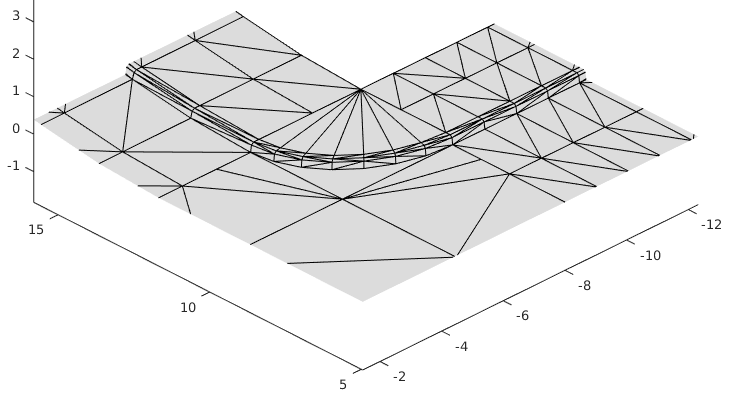
\includegraphics[width=0.6\linewidth]{Figures/mesh_dense}
	\caption{Porzione di \textit{mesh} particolarmente densa di triangoli.}
	\label{meshdense}
\end{figure}
\begin{figure}
	\centering
	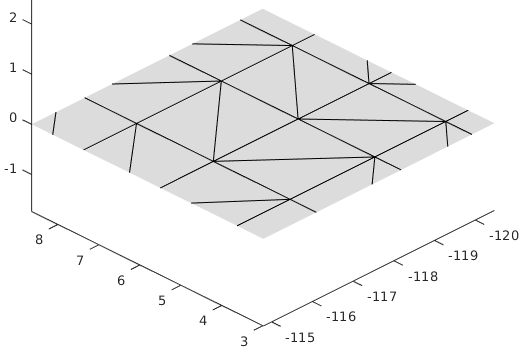
\includegraphics[width=0.6\linewidth]{Figures/mesh_notsodense}
	\caption{Porzione di \textit{mesh} non così particolarmente densa di triangoli.}
	\label{meshnotsodense}
\end{figure}
%
\clearpage
%
\begin{table}
	\centering
	\begin{tabular}{c|c|c|c|}
		\cline{2-4} 
		& \multicolumn{3}{c|}{\textbf{Modello di contatto}} \\
		\cline{2-4} 
		& \textbf{Rill} & \textbf{Ponderato sull'area} & \textbf{\textit{Mix}} \\ 
		\hline
		\multicolumn{1}{|c|}{$T_{totale}$ [ms]} & 116.543 & 121.249 & 106.058 \\ 
		\hline 
		\multicolumn{1}{|c|}{$T_{step}$ [ms]} & 0.0041621 & 0.00433017 & 0.00378765 \\ 
		\hline 
		\multicolumn{1}{|c|}{$\sigma$ [ms$^2$]} & 5.21719e-05 & 3.09234e-06 & 1.11754e-05 \\ 
		\hline
	\end{tabular}
	\\[0.5cm]
	Pneumatico 205/55R16\\
	Campionamenti = 28000\\
	Numero medio di triangoli sotto lo pneumatico = 11.4\\
	\textit{Switch} Rill $\triangleright$ Area a 10 triangoli
	\caption{Tempi per il modello di pneumatico \texttt{MagicFormula} nel caso di \textit{mesh} densa.}
	\label{MFcordolo}
\end{table}
\begin{table}
	\centering
	\begin{tabular}{c|c|c|c|c|c|}
		\cline{2-6} 
		& \multicolumn{2}{c|}{\textbf{Precisione}} &\multicolumn{3}{c|}{\textbf{Modello di contatto}} \\
		\cline{2-6} 
		& \textbf{Dischi} & \textbf{Punti} & \textbf{Campionamento} & \textbf{Ponderato sull'area} & \textbf{\textit{Mix}} \\ 
		\hline
		
		\multicolumn{1}{|c|}{$T_{step}$ [ms]} & 5 & 5 & 0.30604 & 0.027332 & 0.292775 \\ 
		\hline 
		\multicolumn{1}{|c|}{$\sigma$ [ms$^2$]} & 5 & 5 & 0.050355 & 0.0007717 & 0.076598 \\ 
		\hhline{======}
		
		\multicolumn{1}{|c|}{$T_{step}$ [ms]} & 10 & 5 & 0.31406 & 0.029972 & 0.30546 \\ 
		\hline 
		\multicolumn{1}{|c|}{$\sigma$ [ms$^2$]} & 10 & 5 & 0.0165893 & 0.000768059 & 0.038468 \\ 
		\hhline{======}
		
		\multicolumn{1}{|c|}{$T_{step}$ [ms]} & 5 & 10 & 0.38714 & 0.030945 & 0.37890 \\ 
		\hline 
		\multicolumn{1}{|c|}{$\sigma$ [ms$^2$]} & 5 & 10 & 0.039487 & 0.000744563 & 0.085648 \\ 
		\hhline{======}
		
		%%%
		\multicolumn{1}{|c|}{$T_{step}$ [ms]} & 10 & 10 & 0.40604 & 0.031138 & 0.316745 \\ 
		\hline 
		\multicolumn{1}{|c|}{$\sigma$ [ms$^2$]} & 10 & 10 & 0.0104055 & 0.000660589 & 0.0426783 \\ 
		\hhline{======}
		
		\multicolumn{1}{|c|}{$T_{step}$ [ms]} & 10 & 20 & 1.55412 & 0.0563041 & 1.17447 \\ 
		\hline 
		\multicolumn{1}{|c|}{$\sigma$ [ms$^2$]} & 10 & 20 & 0.142766 & 0.000214928 & 0.619357 \\ 
		\hhline{======}
		
		\multicolumn{1}{|c|}{$T_{step}$ [ms]} & 20 & 10 & 0.840434 & 0.0285447 & 0.651595 \\ 
		\hline 
		\multicolumn{1}{|c|}{$\sigma$ [ms$^2$]} & 20 & 10 & 0.0398545 & 5.12437e-05 & 0.193016 \\ 
		\hhline{======}
		 
		\multicolumn{1}{|c|}{$T_{step}$ [ms]} & 20 & 20 & 3.46259 & 0.0587258 & 2.73157 \\ 
		\hline 
		\multicolumn{1}{|c|}{$\sigma$ [ms$^2$]} & 20 & 20 & 0.692889 & 0.000257929 & 3.51893 \\
		\hline
	\end{tabular}
	\\[0.5cm]
	Pneumatico 205/55R16\\
	Campionamenti = 28000\\
	Numero medio di triangoli sotto lo pneumatico = 11.4\\
	\textit{Switch} Area $\triangleright$ Campionamento a 10 triangoli
	\caption{Tempi per il modello di pneumatico \texttt{MultiDisk} nel caso di \textit{mesh} densa.}
	\label{MDcordolo}
\end{table}
%
\clearpage
%
\begin{table}
	\centering
	\begin{tabular}{c|c|c|c|}
		\cline{2-4} 
		& \multicolumn{3}{c|}{\textbf{Modello di contatto}} \\
		\cline{2-4} 
		& \textbf{Rill} & \textbf{Ponderato sull'area} & \textbf{\textit{Mix}} \\ 
		\hline 
		\multicolumn{1}{|c|}{$T_{totale}$ [ms]} & 64.15 & 46.44 & 54.269 \\ 
		\hline 
		\multicolumn{1}{|c|}{$T_{step}$ [ms]} & 0.00229099 & 0.00165851 & 0.00193811 \\ 
		\hline 
		\multicolumn{1}{|c|}{$\sigma$ [ms$^2$]} & 3.92268e-06 & 4.39344e-06 & 5.825e-06 \\
		\hline 
	\end{tabular}
	\\[0.5cm]
	Pneumatico 205/55R16\\
	Campionamenti = 28000\\
	Numero medio di triangoli sotto lo pneumatico = 3.2\\
	\textit{Switch} Rill $\triangleright$ Area a 3 triangoli
	\caption{Tempi per il modello di pneumatico \texttt{MagicFormula} nel caso di \textit{mesh} poco densa.}
	\label{MFpiano}
\end{table}
\begin{table}
	\centering
	\begin{tabular}{c|c|c|c|c|c|}
		\cline{2-6} 
		& \multicolumn{2}{c|}{\textbf{Precisione}} &\multicolumn{3}{c|}{\textbf{Modello di contatto}} \\
		\cline{2-6} 
		& \textbf{Dischi} & \textbf{Punti} & \textbf{Campionamento} & \textbf{Ponderato sull'area} & \textbf{\textit{Mix}} \\ 
		\hline
		
		\multicolumn{1}{|c|}{$T_{step}$ [ms]} & 5 & 5 & 0.29604 & 0.010375 & 0.020880 \\ 
		\hline 
		\multicolumn{1}{|c|}{$\sigma$ [ms$^2$]} & 5 & 5 & 0.00364537 & 0.00734568 & 0.0027406 \\ 
		\hhline{======}
		
		\multicolumn{1}{|c|}{$T_{step}$ [ms]} & 10 & 5 & 0.31406 & 0.015352 & 0.027446 \\ 
		\hline 
		\multicolumn{1}{|c|}{$\sigma$ [ms$^2$]} & 10 & 5 & 0.0174863 & 0.000436738 & 0.0047837 \\ 
		\hhline{======}
		
		\multicolumn{1}{|c|}{$T_{step}$ [ms]} & 5 & 10 & 0.42839 & 0.01972 & 0.038590 \\ 
		\hline 
		\multicolumn{1}{|c|}{$\sigma$ [ms$^2$]} & 5 & 10 & 0.027645 & 0.0045783 & 0.007463 \\ 
		\hhline{======}
		
		%%%
		\multicolumn{1}{|c|}{$T_{step}$ [ms]} & 10 & 10 & 0.213785 & 0.0115888 & 0.0111662 \\ 
		\hline 
		\multicolumn{1}{|c|}{$\sigma$ [ms$^2$]} & 10 & 10 & 0.0021398 & 1.73799e-05 & 2.52509e-05 \\
		\hhline{======}

		\multicolumn{1}{|c|}{$T_{step}$ [ms]} & 10 & 20 & 0.902904 & 0.0210344 & 0.0222986 \\ 
		\hline 
		\multicolumn{1}{|c|}{$\sigma$ [ms$^2$]} & 10 & 20 & 0.0444643 & 4.91353e-05 & 0.000116275 \\ 
		\hhline{======}
		
		\multicolumn{1}{|c|}{$T_{step}$ [ms]} & 20 & 10 & 0.481218 & 0.0114461 & 0.0112381 \\ 
		\hline 
		\multicolumn{1}{|c|}{$\sigma$ [ms$^2$]} & 20 & 10 & 0.0115384 & 2.87254e-05 & 1.70045e-05 \\ 
		\hhline{======}
		
		\multicolumn{1}{|c|}{$T_{step}$ [ms]} & 20 & 20 & 1.88533 & 0.019253 & 0.0193953 \\ 
		\hline 
		\multicolumn{1}{|c|}{$\sigma$ [ms$^2$]} & 20 & 20 & 0.142808 & 2.87459e-05 & 3.20608e-05 \\ 
		\hline
	\end{tabular}
	\\[0.5cm]
	Pneumatico 205/55R16\\
	Campionamenti = 28000\\
	Numero medio di triangoli sotto lo pneumatico = 3.2\\
	\textit{Switch} Area $\triangleright$ Campionamento a 3 triangoli
	\caption{Tempi per il modello di pneumatico \texttt{MultiDisk} nel caso di \textit{mesh} poco densa.}
	\label{MDpiano}
\end{table}
%
\clearpage
\noindent
Testando il modello al simulatore è stato possibile valutare la sua complessità computazionale. Le specifiche tecniche di questo simulatore sono:
\begin{itemize}
	\item sistema operativo: 64bit Concurrent Real-Time RedHawk 7.5 (CentOS 7.5 + RedHawk 4.9.98 Real-Time Kernel);
	\item memoria RAM: 32 GB;
	\item processore: Intel Xeon(R) 3.40 GHz (16 \textit{cores});
	\item scheda grafica: Nvidia GeForce GTX 680.
\end{itemize}
I tempi rilevati per il modello di pneumatico a singolo disco \texttt{MagicFormula} sono riportati nella Tabella \ref{MF}. Analogamente, i tempi rilevati per il modello di pneumatico a più dischi \texttt{MultiDisk} sono riportati nella Tabella \ref{MD}.
%
\begin{table}
	\centering
	\begin{tabular}{c|c|c|}
		\cline{2-3} 
		& \multicolumn{2}{c|}{\textbf{Modello di contatto}} \\
		\cline{2-3} 
		& \textbf{Ponderato sull'area} & \textbf{\textit{Mix}} \\ 
		\hline
		\multicolumn{1}{|c|}{$T_{step}$ [$\mu$s]} & 9.6688 & 9.7658 \\ 
		\hline 
		\multicolumn{1}{|c|}{$\sigma$ [$\mu$s$^2$]} & 1.4018 & 1.4983 \\ 
		\hline
	\end{tabular}
	\\[0.5cm]
	Pneumatico 250/55R11\\
	Campionamenti = 30000\\
	\textit{Switch} Rill $\triangleright$ Area a 10 triangoli
	\caption{Tempi sul simulatore per il modello di pneumatico \texttt{MagicFormula}.}
	\label{MF}
\end{table}
%
\begin{table}
	\centering
	\begin{tabular}{c|c|c|c|c|}
		\cline{2-5} 
		& \multicolumn{2}{c|}{\textbf{Precisione}} &\multicolumn{2}{c|}{\textbf{Modello di contatto}} \\
		\cline{2-5} 
		& \textbf{Dischi} & \textbf{Punti} & \textbf{Ponderato sull'area} & \textbf{\textit{Mix}} \\ 
		\hline
		\multicolumn{1}{|c|}{$T_{step}$ [$\mu$s]} & 5 & 5 & 24.5736 & 39.6069 \\ 
		\hline 
		\multicolumn{1}{|c|}{$\sigma$ [$\mu$s$^2$]} & 10 & 5 & 42.6262 & 439.6915 \\ 
		\hhline{=====}
		
		\multicolumn{1}{|c|}{$T_{step}$ [$\mu$s]} & 5 & 10 & 24.6686 & 55.7135 \\ 
		\hline 
		\multicolumn{1}{|c|}{$\sigma$ [$\mu$s$^2$]} & 10 & 10 & 41.4114 & 479.8682 \\ 
		\hline
	\end{tabular}
	\\[0.5cm]
	Pneumatico 250/55R11\\
	Campionamenti = 30000\\
	\textit{Switch} Area $\triangleright$ Campionamento a 10 triangoli
	\caption{Tempi sul simulatore per il modello di pneumatico \texttt{MultiDisk}.}
	\label{MD}
\end{table}